\chapter{Experimental evaluation} % Main chapter title

\label{Chapter5} % For referencing the chapter elsewhere, use \ref{Chapter5} 

In this section, data exploration, the experimental setup, the metrics for the evaluation between the three algorithms, as well as the result of the experiment are presented.

\section{Data exploration}
\subsection{Descriptive Data Summarization}

In this section, some basic descriptive statistics of the data will be described, in order for the understanding of the overall picture of the data. Figure \ref{fig:boxplot} represent the boxplot diagrams of the energy, speechiness, acousticness, danceability, tempo, instrumentalness, valence, liveness, and loudness respectively. For key, mode, and time signature, as they are categorical variables, boxplot diagram information is not useful. Instead, for these variables, the frequency of the values, such as in table \ref{fig:freq_table} is displayed.

\begin{figure}
  \begin{subfigure}[b]{0.3\textwidth}
    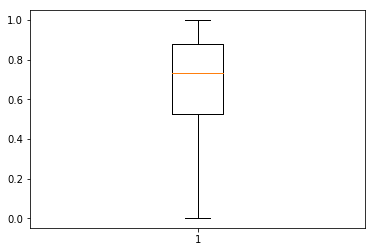
\includegraphics[width=\textwidth]{energy}
    \caption{Energy}
    \label{fig:energy}
  \end{subfigure}
  \hfill
  \begin{subfigure}[b]{0.3\textwidth}
    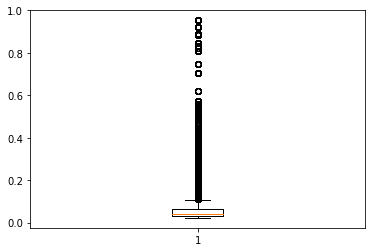
\includegraphics[width=\textwidth]{speechiness}
    \caption{Speechiness}
    \label{fig:speechiness}
  \end{subfigure}
  \hfill
  \begin{subfigure}[b]{0.3\textwidth}
    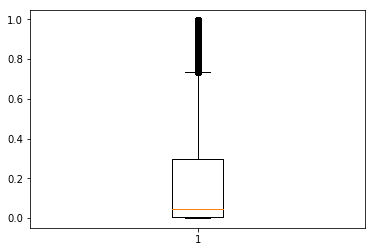
\includegraphics[width=\textwidth]{acousticness}
    \caption{Acousticness}
    \label{fig:acousticness}
  \end{subfigure}
  
  \bigskip
    \begin{subfigure}[b]{0.3\textwidth}
    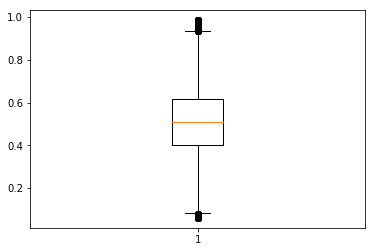
\includegraphics[width=\textwidth]{danceability}
    \caption{Danceability}
    \label{fig:danceability}
  \end{subfigure}
  \hfill
    \begin{subfigure}[b]{0.3\textwidth}
    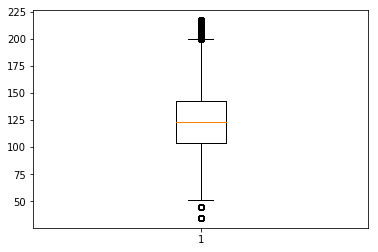
\includegraphics[width=\textwidth]{tempo}
    \caption{Tempo}
    \label{fig:tempo}
  \end{subfigure}
  \hfill
    \begin{subfigure}[b]{0.3\textwidth}
    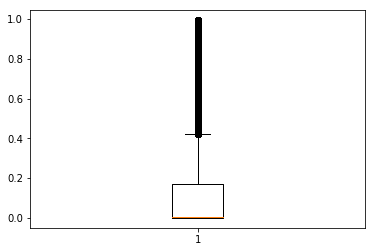
\includegraphics[width=\textwidth]{instrumentalness}
    \caption{Instrumentalness}
    \label{fig:instrumentalness}
  \end{subfigure}
  
  \bigskip
      \begin{subfigure}[b]{0.3\textwidth}
    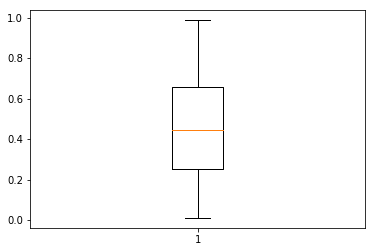
\includegraphics[width=\textwidth]{valence}
    \caption{Valence}
    \label{fig:valence}
  \end{subfigure}
  \hfill
    \begin{subfigure}[b]{0.3\textwidth}
    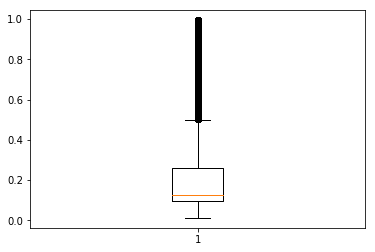
\includegraphics[width=\textwidth]{liveness}
    \caption{Liveness}
    \label{fig:liveness}
  \end{subfigure}
  \hfill
    \begin{subfigure}[b]{0.3\textwidth}
    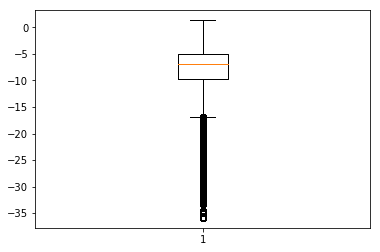
\includegraphics[width=\textwidth]{loudness}
    \caption{Loudness}
    \label{fig:loudness}
  \end{subfigure}
  
  \caption{Boxplot diagram of music features}
  \label{fig:boxplot}
\end{figure}

\begin{figure}
  \begin{subfigure}[b]{0.3\textwidth}
    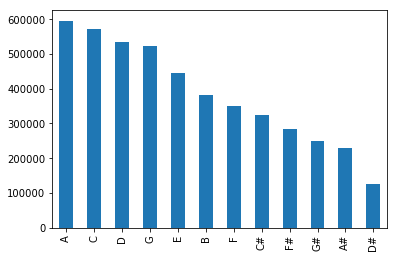
\includegraphics[width=\textwidth]{key}
    \caption{Key}
    \label{fig:key}
  \end{subfigure}
  \hfill
   \begin{subfigure}[b]{0.3\textwidth}
    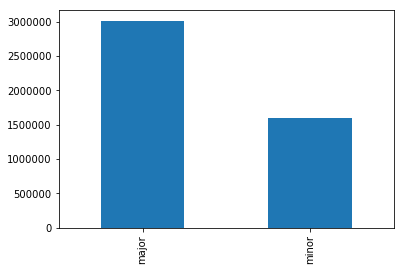
\includegraphics[width=\textwidth]{mode}
    \caption{Mode}
    \label{fig:mode}
  \end{subfigure}
  \hfill
  \begin{subfigure}[b]{0.3\textwidth}
    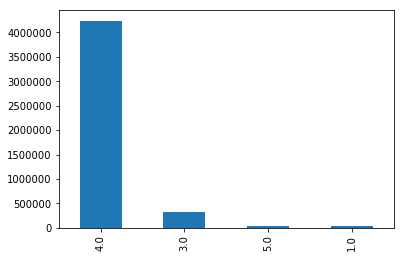
\includegraphics[width=\textwidth]{time_signature}
    \caption{Time signature}
    \label{fig:time_signature}
  \end{subfigure}
	
	\caption{Frequency table of music features}
	\label{fig:freq_table}
\end{figure}

\bigskip

\noindent We can see that from the diagrams:
\begin{itemize}
	\item Energy: the median is quite high, at nearly 0.8. However, the interquartile range of the energy is 0.35, suggesting that the energy spans equally across the value range.
	\item Speechiness: the median is at 0.04, with the first quartile at 0.03 and third quartile at 0.06, showing that most of the tracks have low level of spoken word. 
	\item Acousticness: the median is also at 0.04, with the first quartile at 0.003. However, the third quartile is at 0.3, suggesting that most of the tracks are not acoustic.
	\item Danceability: the median is at 0.5, with the first quartile at 0.4 and third quartile at 0.6, showing a normal distribution, which means that people listen equally to danceable track as well as undanceable track.
	\item Tempo: the median tempo is 123, with the first quartile of 104 and third quartile of 142, suggesting that most people listen to Allegro, which is fast and bright music.
	\item Instrumentalness: the median of 0.003 and the third quartile of 0.17 imply that most of the tracks contain vocal and not just pure instrument.
	\item Valence: with the median of 0.44, first quartile of 0.25, and third quartile of 0.66, valence also forms the normal distribution, suggesting that people listen equally to both positive and negative music.
	\item Liveness: the median of 0.12 and third quartile of 0.25 indicate that most tracks have a low level of liveness.
	\item Loudness: the first quartile of -9 and third quartile of -5 implement that most song have quite the same level of loudness.
	\item Key: songs with different key have different playing frequency. Overall, major key songs dominate minor ones.
	\item Mode: major key tracks are played more than minor ones, as previously stated.
	\item Time signature: the table indicates that more than 90\% of the tracks have 4 beats in each measure, around 7\% of the tracks have 3 beats in each measure, and the rest of the track have either 1 or 5 beats per measure.
\end{itemize}
	
\subsection{Data Clustering}
Cluster analysis is applied to the dataset to discover whether users listening behavior can be split into different groups. For each user, the average of the features of the tracks that user listen to is taken. After that, K-Mean algorithms is applied to the dataset to derive the clusters. Silhouette coefficient, shown in figure \ref{fig:Silhouette}, and Sum of Squared Errors, shown in figure \ref{fig:SSE} recommends the chosen of 6 for the number of clustering. 

\begin{figure}
	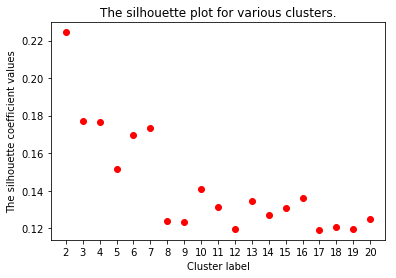
\includegraphics[width=8cm]{silhouetteall_8}
	\centering
	 \caption{Silhouette coefficient of the dataset for different number of clusters}
    \label{fig:Silhouette}
\end{figure}

\begin{figure}
	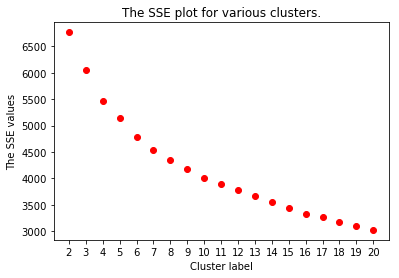
\includegraphics[width=8cm]{SSEall_8}
	\centering
	 \caption{SSE of the dataset for different number of clusters}
    \label{fig:SSE}
\end{figure}

\noindent The detail of each feature of the clustering is shown in figure \ref{fig:boxplot_cluster}. The result demonstrates a trivial contrast between the clusters; However, there are still some differentiable characteristics between the clusters:

\begin{itemize}
\item[•] The first cluster has a high level of acousticness, instrumentalness,  and tempo, whereas a low level of energy, liveness, speechiness, and loudness, suggesting that this group favors recording acoustic music with fast pace.

\item[•] The second cluster has a very high level of energy, liveness, loudness, speechiness, and valence, while the level of acoustiness, instrumentalness, and tempo remain low, implies that the user of this group might favor loud, bright live electronic music.

\item[•] The third cluster is characterized by low danceability and valence, suggesting that these users tend to listen to more negative music than other users.

\item[•] The fourth cluster has similar characteristics as the third cluster, but with higher level of acousticness and lower level of energy, suggesting that the users in this group also listen to acoustic negative music.

\item[•] The fifth cluster is characterized by low acousticness and instrumentalness. By contrast, it has high energy, loudness, tempo, and valence, suggesting that users of the group often listen to fast and happy tracks.

\item[•] The final cluster has the highest danceability and valence among the groups, implies that the users listen to dancing music. 
\end{itemize} 


\begin{figure}
  \begin{subfigure}[b]{0.3\textwidth}
    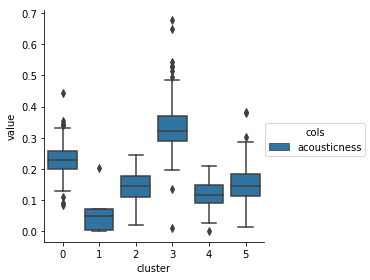
\includegraphics[width=\textwidth]{clusterting_acousticness}
    \caption{Acousticness}
    \label{fig:clusterting_acousticness}
  \end{subfigure}
  \hfill
  \begin{subfigure}[b]{0.3\textwidth}
    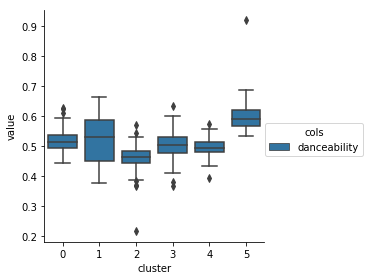
\includegraphics[width=\textwidth]{clusterting_danceability}
    \caption{Danceability}
    \label{fig:clusterting_danceability}
  \end{subfigure}
  \hfill
  \begin{subfigure}[b]{0.3\textwidth}
    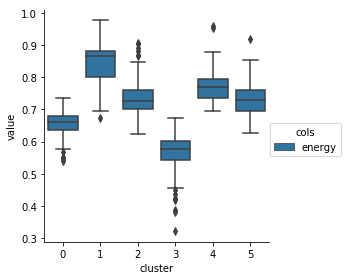
\includegraphics[width=\textwidth]{clusterting_energy}
    \caption{Energy}
    \label{fig:clusterting_energy}
  \end{subfigure}
  
  \bigskip
    \begin{subfigure}[b]{0.3\textwidth}
    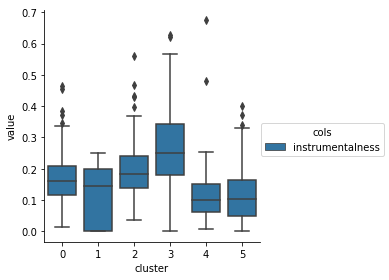
\includegraphics[width=\textwidth]{clusterting_instrumentalness}
    \caption{Instrumentalness}
    \label{fig:clusterting_instrumentalness}
  \end{subfigure}
  \hfill
    \begin{subfigure}[b]{0.3\textwidth}
    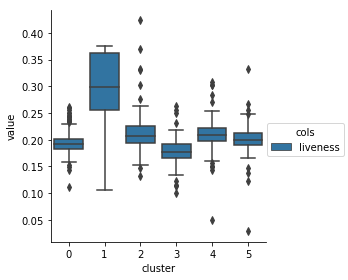
\includegraphics[width=\textwidth]{clusterting_liveness}
    \caption{Liveness}
    \label{fig:clusterting_liveness}
  \end{subfigure}
  \hfill
    \begin{subfigure}[b]{0.3\textwidth}
    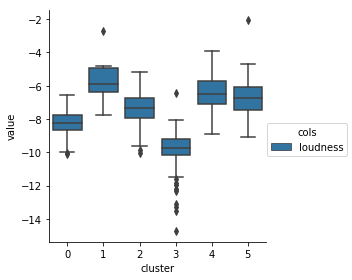
\includegraphics[width=\textwidth]{clusterting_loudness}
    \caption{Loudness}
    \label{fig:clusterting_loudness}
  \end{subfigure}
  
  \bigskip
      \begin{subfigure}[b]{0.3\textwidth}
    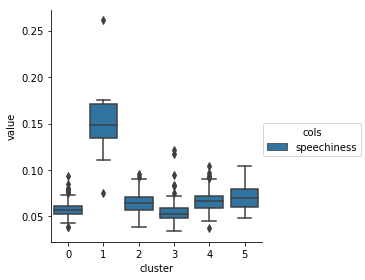
\includegraphics[width=\textwidth]{clusterting_speechiness}
    \caption{Speechiness}
    \label{fig:clusterting_speechiness}
  \end{subfigure}
  \hfill
    \begin{subfigure}[b]{0.3\textwidth}
    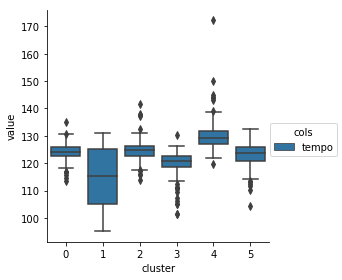
\includegraphics[width=\textwidth]{clusterting_tempo}
    \caption{Tempo}
    \label{fig:clusterting_tempo}
  \end{subfigure}
  \hfill
    \begin{subfigure}[b]{0.3\textwidth}
    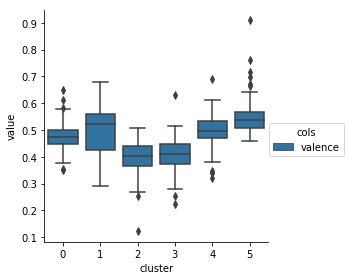
\includegraphics[width=\textwidth]{clusterting_valence}
    \caption{Valence}
    \label{fig:clusterting_valence}
  \end{subfigure}
  
  \caption{Boxplot diagram of different clusters}
  \label{fig:boxplot_cluster}
\end{figure}

\section{Experimental Setup}
The main goal of this experiment is to measure how well the learning to rank algorithm is using the described dataset, taking the two remaining algorithms as the baseline. 

\noindent The two baseline algorithms used to compare with the learning to rank algorithm is the two that were mentioned in Chapter \ref{Chapter3}. The first one is the na\"ive collaborative filtering, which is the most simple and straightforward collaborative filtering method. The second one is the matrix factorization CF for implicit feedback dataset, which is the state-of-the-art collaborative filtering. The algorithm applies two different weighting strategies: one with a constant weighting scheme, while the other uses BM25 weight scheme \cite{singhal2001modern}.

\noindent For the ranking algorithm, two versions are setup: with and without item features. For the one with item features, the features are converted from continuous to categorical values, using the following rules:

\begin{itemize}
	\item Acousticness, danceability, energy, instrumentalness, liveness, speechiness, valence: the features are divided equally into 5 bins, each has range of 0.2.
	\item Key: each key represent a category on its own.
	\item Loudness: the feature is divided equally into 12 categories, each has range of 5.
	\item Tempo: tempo is categorized using standard Italian tempo markings \cite{2018Tempo}. In details, the feature is divided into these following categories:
	\begin{itemize}
		\item Grave: tempo from 40 to 50 beat per minute (bpm).
		\item Largo: tempo from 50 to 55 bpm.
		\item Larghetto: tempo from 55 to 60 bpm.
		\item Adagio: tempo from 60 to 70 bpm.
		\item Andante: tempo from 70 to 85 bpm.
		\item Moderato: tempo from 85 to 100 bpm.
		\item Allegretto: tempo from 100 to 115 bpm.
		\item Allegro: tempo from 115 to 140 bpm.
		\item Vivace: tempo from 140 to 150 bpm.
		\item Presto: tempo from 150 to 170 bpm.
		\item Prestissimo: tempo higher than 170 bpm.
\end{itemize}	  
\end{itemize}

As there are many hyperparameters in both implicit and ranking algorithm, a sequential optimization strategy using decision trees is used to optimize the hyperparameters \cite{ForestMinimize2018}. The model is improved by sequentially evaluating the expensive function at the next best point, thereby finding the best hyperparameters with as few evaluations as possible. 

To reduce training time and approximate the best practice predicting time, instead of implementing the algorithms from scratch, I used a Python library developed by Benfred \cite{Benfred2018} for the implicit algorithm, and LightFM library \cite{DBLP:conf/recsys/Kula15} for the ranking algorithm.

\section{Score Metrics}
In this experiment, Average Precision (AP) is used to evaluate the efficiency of the algorithms. AP is defined as follow \cite{liu2009learning}:

\begin{displaymath}
AP(q) = \frac{\sum_{k=1}^m P@k(q) \cdot l_k}{\#\text{\{relevant documents\}}}
\end{displaymath}

\noindent with \( P@k \) is precision at K:

\begin{displaymath}
P@k(q) = \frac{\#\text{\{relevant documents in the top k positions\}}}{k}
\end{displaymath}

\noindent where \(m\) is the total number of document associated with query q, and \(l_k\) is the binary judgment on the relevance of the document at the \(k\)-th position. For this experiment, AP with value \(k = 1, 2, 3, 4, 5, \text{and } 10\) is measured, as we want to observe the behavior of the algorithms on optimizing for the top items. 

\section{Experiment Result}
\subsection{Accuracy}
The Average Precision of the algorithms is demonstrated in figure \ref{AP_result}. The na\"ive collaborative filtering has the poorest performance among the algorithms, with the Average Precision being 0.25 when \(k = 1\) and decreases to 0.2 when \(k = 5\), while the other two algorithms show comparable results. The learning to rank algorithm, optimizing for top items, has a slightly better precision compare to the implicit algorithm for \(k = 1 \text{ and } 2\). As \(k\) increases, the precision of all algorithms declines. The result demonstrates that adding Spotify music features does not increase the accuracy of the algorithm. 

\begin{figure}[h]
	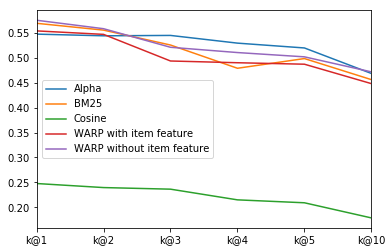
\includegraphics[width=8cm]{result}
	\centering
	\caption{Average Precision of the algorithms}
	\label{AP_result}
\end{figure}

\noindent A detail study of the behavior of each algorithms regarding different sample size is demonstrate in figure \ref{AP_with_training_size_result}. In most cases, the precision of all algorithms starts off low and builds up as the training size increases, attaining their peak accuracies as the training size grows to around 600,000, then remaining stable regardless of the continuously growing training set.

\begin{figure}[htbp]
  \begin{subfigure}[b]{0.3\textwidth}
    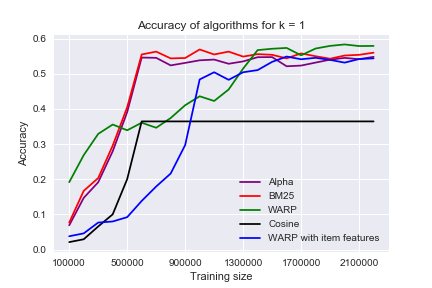
\includegraphics[width=\textwidth]{pop1}
    \caption{Average Precision of the algorithms with k = 1}
    \label{fig:pop1}
  \end{subfigure}
  \hfill
  \begin{subfigure}[b]{0.3\textwidth}
    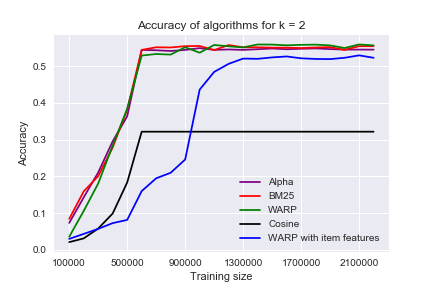
\includegraphics[width=\textwidth]{pop2}
    \caption{Average Precision of the algorithms with k = 2}
    \label{fig:pop2}
  \end{subfigure}
  \hfill
  \begin{subfigure}[b]{0.3\textwidth}
    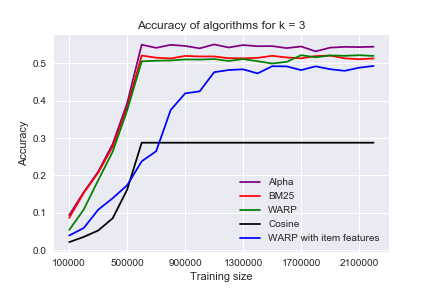
\includegraphics[width=\textwidth]{pop3}
    \caption{Average Precision of the algorithms with k = 3}
    \label{fig:pop3}
  \end{subfigure}
  
   \bigskip
    \begin{subfigure}[b]{0.3\textwidth}
    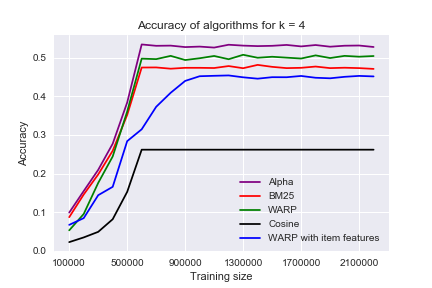
\includegraphics[width=\textwidth]{pop4}
    \caption{Average Precision of the algorithms with k = 4}
    \label{fig:pop4}
  \end{subfigure}
  \hfill
    \begin{subfigure}[b]{0.3\textwidth}
    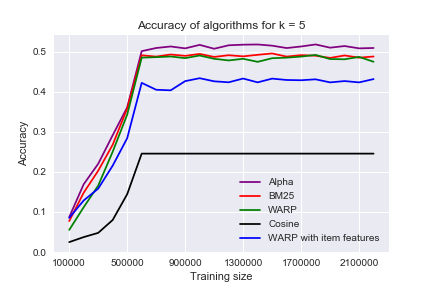
\includegraphics[width=\textwidth]{pop5}
    \caption{Average Precision of the algorithms with k = 5}
    \label{fig:pop5}
  \end{subfigure}
  \hfill
  \caption{Average Precision of the algorithms regarding training size}
  \label{AP_with_training_size_result}
\end{figure} 

\subsection{Computational expense}
Both the na\"ive collaborative filtering and the implicit collaborative filtering have linear time complexity, meaning that training time increases linearly as the number of user and item increase. The time complexity of the learning to rank algorithm, on the other hand, is \( \mathcal{O} (Y + d) \cdot D ) \), with \(Y\) is the number of classes, \(d\) is the average number of non-zero values per user array, and \(D\) is the size of the embedding space. 

\noindent A summary of the training of various algorithms is shown in figure \ref{training_time}. As the time complexity of the learning to rank algorithm is independent of the training size, training time is stable regardless of the number of entity in the dataset. Adding item features makes training time accrues as the computational complexity to optimize the rank increase; However, a careful selection of feature would shorten training time and make it invariable as training size increase. The training time of the implicit CF in this case is quite low as a result of the small size of the dataset; Nonetheless, as the size increase, training time would also linearly build up.

\begin{figure}[h]
	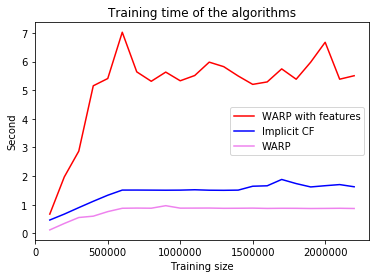
\includegraphics[width=8cm]{times_complexity}
	\centering
	\caption{Training time of the algorithms}
	\label{training_time}
\end{figure}
